\chapter{Fundamenta Teórica}
Neste capítulo serão apresentados os conceitos
abordados neste trabalho. O problema inverso será apresentado
em linhas gerais e o leitor tomará conhecimento do processo de inversão sísmica.
Serão apresentados os conceitos relacionados a \textit{Deep Learning}, assim como os
elementos de redes neurais convolucionais. Esta fundamentação
teórica é relevante para o entendimento de como o modelo de rede neural convolucional
pode ser adotado para obter ganho qualitativo e quantitativo no pós-processamento
da inversão sísmica.

\section{Problema Inverso}

A teoria de inversão é utilizada em diversas áreas para inferir os valores de
parâmetros relacionados com processos importantes a partir dos dados medidos,
também chamados de dados experimentais. É possível descrever o problema inverso
como o processo de obter informações de um sistema parametrizado, a partir de
dados observáveis, das relações teóricas dos observáveis com os parâmetros não
observáveis e do conhecimento \textit{a priori} sobre os dados não observáveis.

Um sistema físico depende do domínio em estudo. Pode ser uma galáxia para um
astro-físico, pode ser a Terra para um geofísico ou uma partícula quântica
para um físico quântico. O procedimento científico para o estudo de um sistema
físico pode ser dividido em três passos: a parametrização do sistema, a modelagem direta e a modelagem inversa.
A parametrização do sistema se refere à definição do conjunto mínimo de elementos cujos
valores caracterizam completamente o sistema. A modelagem direta se refere concerne a
definição das leis físicas que permitem realizar previsão de dados observáveis, dados
valores dos parâmetros do modelo. A modelagem inversa, por sua vez, se caracteriza pelo
uso de resultados atuais das medições dos parâmetros físicos observáveis, para inferir os valores atuais dos
parâmetros do modelo.

Resolver o problema direto significa prever os valores dos parâmetros observáveis (dados $d$),
que correspondem a um dado modelo (conjunto de parâmetros $m$). Esta predição pode ser denotada
pela Eq. \ref{eq:frdmdl}. Onde $F(.)$ é chamado operador direto.
\begin{equation}
\label{eq:frdmdl}
F(m) = d 
\end{equation}
No exemplo do eletrocardiograma citado anteriormente, o problema direto pode
ser entendido como o cálculo do potencial em algum ponto da superfície da pele,
dados valores conhecidos da atividade elétrica do coração.
O problema inverso pode ser descrito em uma forma discreta como:
\begin{equation}
\label{eq:deqgm}
m = F^{-1}(d)
\end{equation}
onde, F é p sistema físico investigado e que relaciona os parâmetros do modelo $m=(m_1, m_2,...,m_n) \subset R^n$
estimado que pertence a um conjunto de modelos $M$ admissíveis
em termos de conhecimento prévio (\textit{a priori}), com os dados observados $d \in R^s$.
Na prática $d$ pode ser uma função no domínio do tempo e/ou espaço, ou pode ser
uma coleção de observações discretas. Uma questão relevante é a presença de
ruído nas observações.

\section{Inversão Sísmica}

Os métodos geofísicos frequentemente envolvem a solução e avaliação de problemas inversos,
pois permitem inferir a distribuição das propriedades físicas na subsuperfície da Terra
usando observações da superfície. A inversão sísmica tem um papel fundamental na solução 
de problemas geofísicos, em especial na caracterização de reservatórios \cite{Bosch2010} \cite{Srivastava2009}.
Do ponto de vista prático, as soluções para o problema de inversão sísmica melhora a exploração e
o gerenciamento na indústria petrolífera, pois os dados sísmicos estimados possuem forte correlação com as
propriedades petrofísicas (porosidade, densidade, etc) das rochas da subsuperfície\cite{Figueiredo2014}.

O método de aquisição sísmica de reflexão utiliza
pulsos sísmicos de uma fonte artificial controlada e monitora a resposta em
função do tempo. Neste sistema, cada região de contato entre dois tipos de rochas
diferentes gera reflexão e refração do pulso sísmico, como demonstrado na Figura
\ref{fig:1sismica}.
De um ponto de vista bastante elementar, é possível imaginar que a parte refletida da onda se
propaga em todas as direções, de modo que os componentes horizontal e vertical podem ser obtidos.
O componente horizontal (\textit{s-wave}), referente à reflexão horizontal
da onda, é utilizada no processo de inversão conhecido como inversão elástica. Por outro lado, os componente
vertical da onda (\textit{p-wave}), referente à reflexão vertical do pulso do pulso emitido, é utilizado no processo
conhecido como inversão acústica.

\begin{figure}[ht!]
\begin{center}
  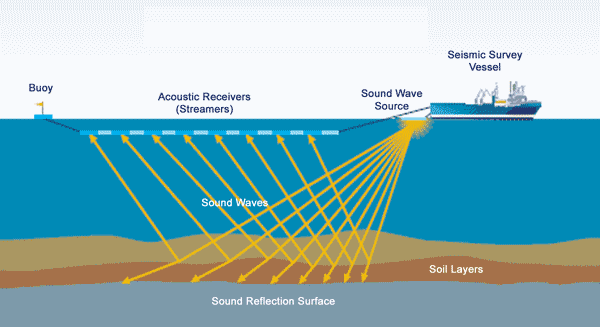
\includegraphics[width=0.8\textwidth]{fig/seismic_survey}
  \caption{Método de sísmica de reflexão \citep{figsismica}}
  \label{fig:1sismica}
\end{center}
\end{figure}

O pulso de onda emitido durante a aquisição possui um formato próprio, uma identidade, e
é conhecido como \textit{wavelet}. É possível imaginar, então, que a resposta obtida
é composta em parte por esta identidade e, em parte, pela característica da região de contato
entre duas camadas de rochas diferentes, na qual ocorreceu a reflexão, acrescentada de um ruído aleatório. Esta característica
é chamada de coeficiente de refletividade.
O dado sísmico utilizado na inversão acústica é uma aproximação da resposta da camada terrestre convolucionada com
a wavelet de aquisição cujo ângulo de incidência é de $90^\circ$ e o valor de refletividade entre as camadas da subsuperfície
com reflexão também de $90^\circ$, definida pela equação \ref{eq:refletv}. Por este motivo, este modelo é chamado convolucional.

\begin{equation}
r(t) = \frac{z(t+\delta t)-z(t)}{z(t+\delta t)+z(t)}
\label{eq:refletv}
\end{equation}

Na equação \ref{eq:refletv}, $z(t)$ é a impedância acústica no tempo $t$ definida por
$z(t)=\rho(t)v(t)$, onde $\rho(t)$ é a densidade da rocha e $v(t)$ a
velocidade de propagação da onda acústica. Com os coeficientes de
reflexão e a discretização da medida de tempo, é possível
modelar o dado sísmico $d(t)$ aplicando a convolução $\otimes$
da \textit{wavelet} $s$ com os coeficientes de refletividade $r$:

\begin{equation}
d(t) = s(\tau) \otimes \sum{j-1}{N} r(t- t_j) \delta(t - t_j) + e_d(t)
\end{equation}
onde $N$ é o número
total de camadas, $e_d(t)$ representa o ruído aleatório em função do tempo
e cada $d_{xy}$ é chamado de traço sísmico. Um conjunto de traços
sísmicos também é chamado de uma imagem, seção ou cubo, no caso de um
levantamento 3D. A \textit{wavelet} ideal seria um pulso tipo delta contendo
todas as frequências, entretanto, na prática as
\textit{wavelets} são pulsos de banda limitada entre $6Hz$ e $65Hz$, o que
limita a frequência da sísmica e sua resolução \citep[p. 11]{sen_livro}.
Como consequência, as imagens resultantes do processo de inversão também terão
o seu espectro de frequência limitado.
A Figura \ref{fig:wavelet} ilustra uma \textit{wavelet} típica extraída de dados
reais.

\begin{figure}[htp]
\begin{center}
  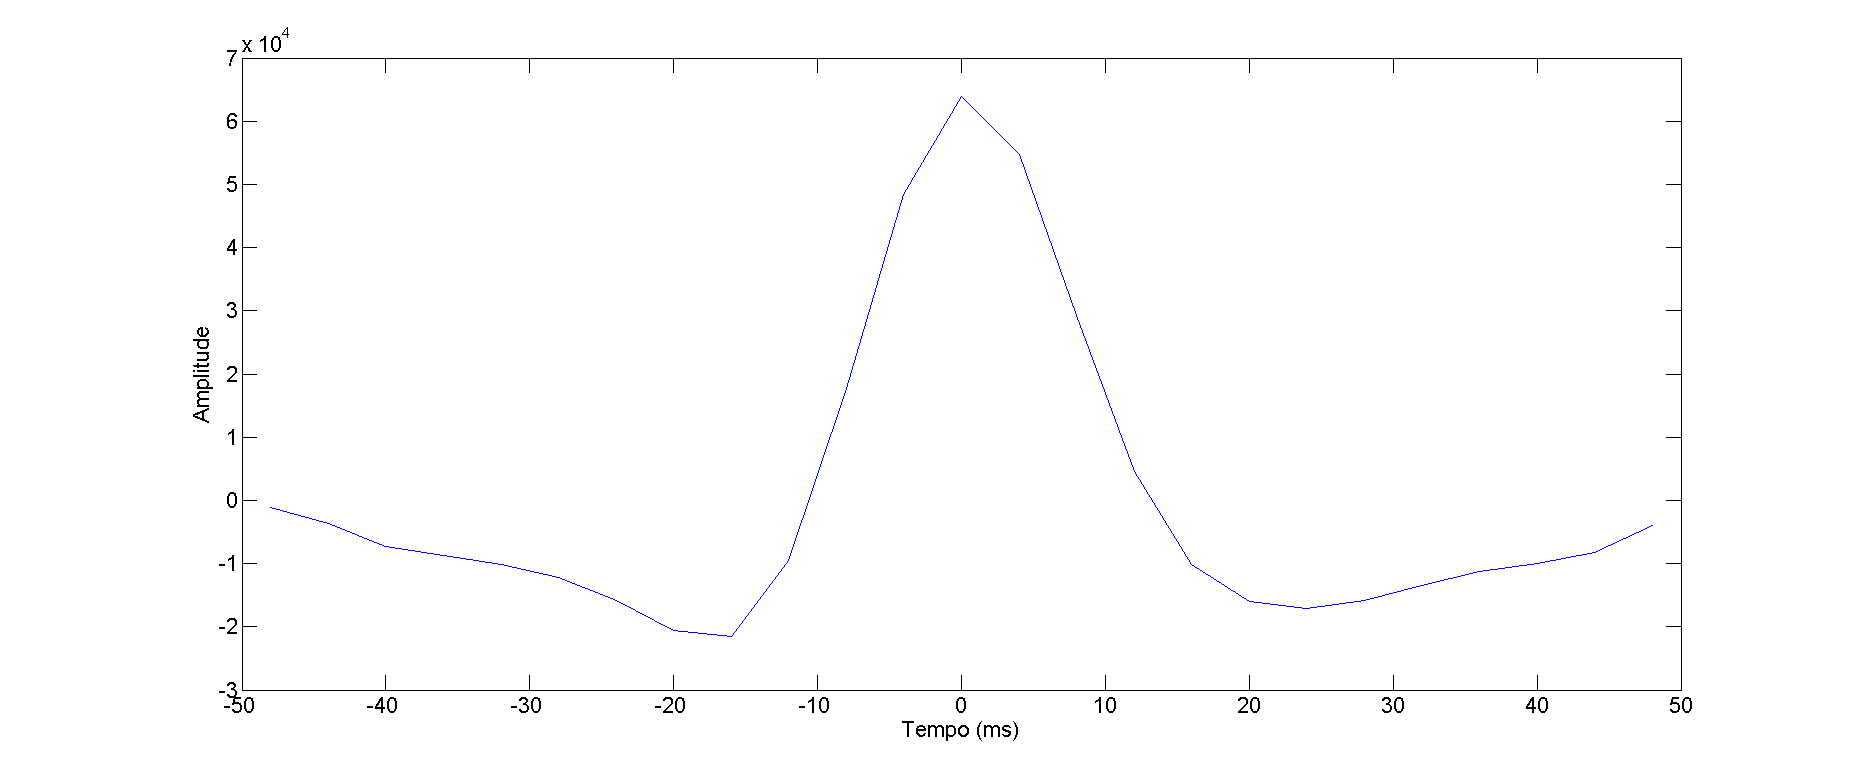
\includegraphics[width=0.8\textwidth]{fig/wavelet}
  \caption{\textit{Wavelet} extraída de dados reais}
  \label{fig:wavelet}
\end{center}
\end{figure}

\section{Deep Learning}


\section{Redes Neurais Convolucionais}
Nesta seção serão apresentados os principais conceitos relacionados às redes
neurais convolucionais, sua estrutura e as principais
aplicações deste modelo de aprendizagem de máquina.

As Redes Neurais Convolucionais (CNN), também chamadas de redes convolucionais,
são um tipo de rede neural especializada em processamento de dados que possuem uma
topologia conhecida e em forma de grade. Exemplos deste tipo de dado são as séries
temporais, que podem ser vistas como uma grade em uma dimensão (1D) com amostras
em intervalos de tempo regulares, e dados de imagem, que podem ser pensados como
uma grade 2D de \textit{pixels}. Entretanto, as redes convolucionais não são restritas
apenas ao processamento visual, elas têm sido empregadas com sucesso, por exemplo,
em reconhecimento de voz e processamento de linguagem natural.
Este modelo de rede é chamada convolucional, pois emprega a operação de convolução
no lugar de multiplicação de matrizes, em pelo menos uma de suas camadas.

A estrutura mais importante de uma CNN é a camada convolucional. Esta, é organizada
de modo a fazer com que cada um dos seus neurônios esteja conectado a um 
pequeno grupo de \textit{pixels} da camada de entrada (figura \ref{fig:cnn_arq}) e não a todos os \text{pixels}, como
ocorre em redes neurais tradicionais. Cada neurônio da camada seguinte se conecta apenas a neurônios
contidos em uma pequena região da camada anterior e assim sucessivamente, esta região que define
o grupo de neurônios conectados ao neurônio da próxima camada é chamada \textbf{campo perceptivo}. Esta arquitetura permite o
aprendizado de características de baixo nível na primeira camada e de características de mais alto nível
nas camadas seguintes.

\begin{figure}[htp]
\begin{center}
  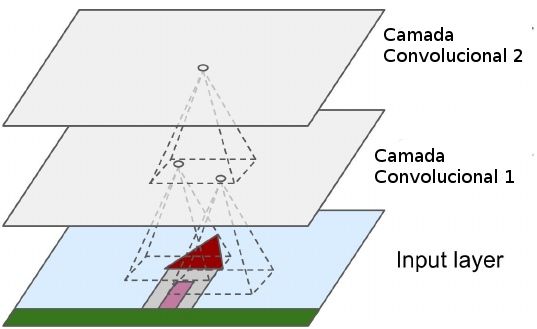
\includegraphics[width=0.8\textwidth]{fig/cnn_arq}
  \caption{Camadas de uma CNN com campos receptivos retangulares.}
  \label{fig:cnn_arq}
\end{center}
\end{figure}

\subsection{Convolução}
A operação de convolução é definida como a integral do produto de duas funções após uma delas sofrer um
certo deslocamento. Considere um exemplo em que se deseja rastrear a localização de uma
nave espacial com um sensor a lazer. O sensor disponibiliza uma saída $x(t)$ referente à posição da nave
no tempo $t$. Ambos, $x$ e $t$, são valores reais, de modo que uma saída diferente pode ser obtida
em qualquer instante de tempo. Considerando que o sensor possui um certo ruido, para realizar uma
estimativa mais precisa da posição da nave é possível ponderar várias medidas de posição juntas.
Como os valores medidos mais recentemente são mais relevantes, é possível utilizar uma função peso
$w(a)$, onde $a$ é o tempo de medição, para fazer uma estimativa ponderada. Se esta média ponderada for aplicada a todos os instantes,
a estimativa de posição da nave será suavizada:

\begin{equation}
 s(t) = \int{x(a) w(t-a)da}
 \label{eq:1}
\end{equation}

A operação de convolução costuma ser denotada com um asterisco (Eq. \ref{eq:2}) e utilizada com o tempo
discretizado, de modo que o tempo $t$ é assumido como valores inteiros:
\begin{equation}
 s(t) = (x * w)(t) = \sum{a=-\inf}{\inf}{x(a)w(t-a)}
 \label{eq:2}
\end{equation}

No contexto das redes convolucionais, $x$ se refere ao conjunto de imagens de entrada, uma sequência multidimensional
de dados, e $w$ é denominado \textit{kernel} ou filtros, uma sequência multidimensional de parâmetros 
a serem otimizados pelo algoritmo de aprendizagem.
Nos casos em que o problema compreende imagens $I$ e filtros $K$ utilizados em duas dimensões:

\begin{equation}
 S(i,j) = (I*K)(i,j) = \sum{m}\sum{n}{I(m,n)K(i-m,j-n)}
\end{equation}

\subsection{Filtros}
Os pesos dos neurônios em uma camada convolucional podem ser representados como uma pequena
imagem do tamanho do campo receptor. Estes filtros (pesos) são os elementos
convolvidas com a imagem de entrada para obter o resultado da camada convolucional.
A figura \ref{fig:conv_filt} ilustra dois conjuntos de pesos possíveis. O primeiro é um quadrado preto
(\textit{pixel} de valor 0) contendo uma coluna central branca (\textit{pixels} com valor 1). 
Analogamente, o segundo filtro é um quadrado preto contendo uma linha central branca.
É possível notar na imagem da esquerda que as linhas verticais brancas se tornaram mais evidentes enquanto o restante
se tornou mais borrado. De modo análogo, na imagem da direita, a convolução com o filtro horizontal evidenciou as linhas brancas horizontais, enquanto que
o restante ficou borrado. Assim, ao convolver uma entrada com o mesmo conjunto de filtros da camada convolucional, se obtém
o mapa de características (feature map).
\begin{figure}[htp]
\begin{center}
  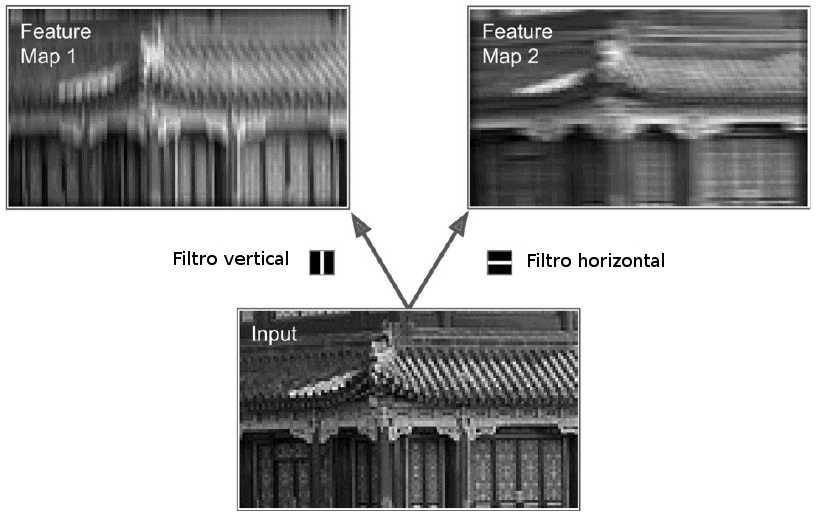
\includegraphics[width=0.7\textwidth]{fig/conv_filt}
  \caption{Aplicação de dois filtros diferentes para obter mapas de características.}
  \label{fig:conv_filt}
\end{center}
\end{figure}

O exemplo anterior apresenta a convolução de uma imagem com dois filtros possíveis, em uma representação 2D.
Entretanto, em situações reais a camada convolucional possui muitos mapas de características, resultando
em uma representação em 3D como ilustrado na figura \ref{fig:featmaps}. O mapa de características de uma camada convolucional
é o resultado da convolução de uma das imagens de entrada com os diversos filtros específicos desta camada,
os quais são iniciados, na maior parte dos casos, aleatoriamente. Na figura estão ilustrados os mapas para a convolução
com apenas uma imagem, de modo que é possível imaginar que à medida que o número de imagens aumenta, a
estrutura ilustrada se replica horizontalmente. 
\begin{figure}[htp]
\begin{center}
  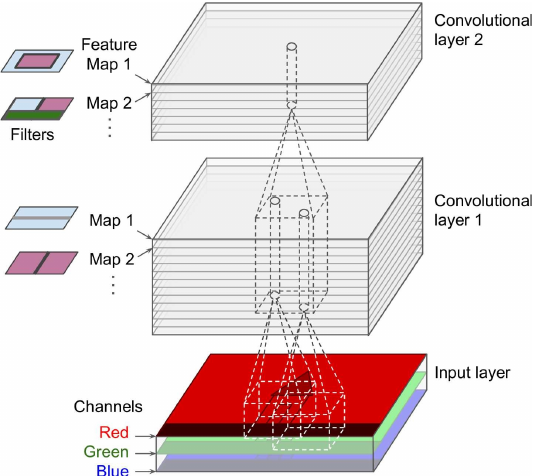
\includegraphics[width=0.7\textwidth]{fig/feat_maps}
  \caption{Camadas convolucionais com múltiplos mapas de características e imagens com três canais.}
  \label{fig:featmaps}
\end{center}
\end{figure}

As redes convolucionais se sustentam sobre três pilares: interações esparsas, compartilhamentos
de parâmetros e representações equivalentes. 
As interações esparsas, também chamadas de conectividade esparsa ou pesos esparsos,
ocorre quando os filtros possuem  dimensão menor que a entrada, ou seja a
dimensão do campo receptivo é menor que a dimensão das imagens de entrada.
De um ponto de vista prático,
a imagem de entrada pode ter milhares de \textit{pixels}, entretanto, é 
possível detectar apenas pequenas regiões com características de maior relevância
com filtros que compreendam apenas algumas dezenas ou centenas de \textit{pixels} na imagem.
Por exemplo, é possível identificar características de uma face humana na identificação de pessoas, ou estruturas com
significado geológico em um estudo geofísico. Como consequência,
menos parâmetros são armazenados e há um ganho na eficiência estatística do
modelo. As figuras \ref{fig:full} e \ref{fig:sparse} ilustram
os modelos de sem conectividade esparsa e com conectividade esparsa, respectivamente.
É possível notar que na conectividade tradicional (figura \ref{fig:full}) todos os elementos da camada inferior
afetam o elemento em destaque $s_3$ da camada seguinte, enquanto que na conectividade esparsa (figura \ref{fig:sparse}) apenas
três elementos afetam o elemento em destaque. O número de elementos que afetam o elemento em destaque na
conectividade esparsa é definido pelo tamanho do filtro utilizado na convolução.

\begin{figure}[htp]
\begin{subfigure}{.5\textwidth}
  \centering
  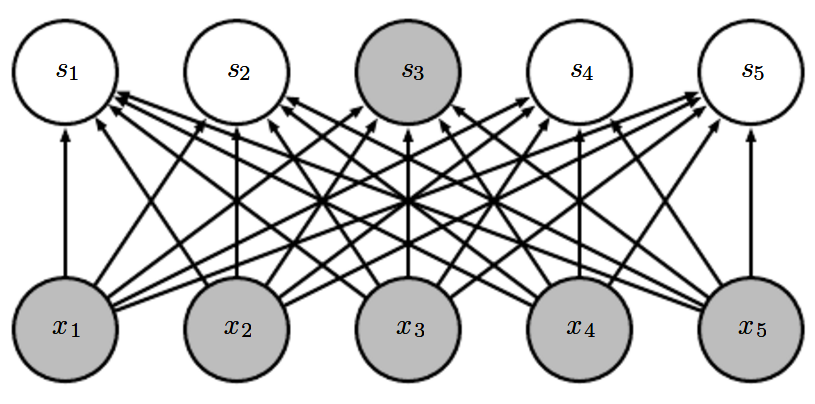
\includegraphics[width=.9\linewidth]{fig/full}
  \caption{Conectividade tradicional.}
  \label{fig:full}
\end{subfigure}%
\begin{subfigure}{.5\textwidth}
  \centering
  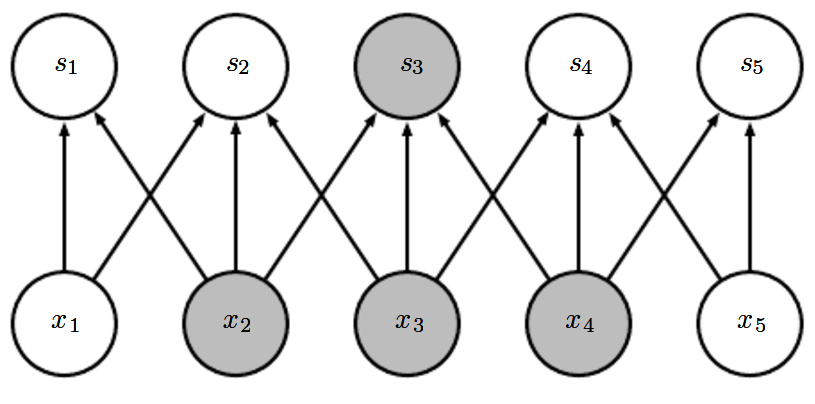
\includegraphics[width=.9\linewidth]{fig/sparse}
  \caption{Conectividade esparsa.}
  \label{fig:sparse}
\end{subfigure}
\end{figure}

O \textbf{compartilhamento de parâmetros}, também chamado de \textbf{pesos amarrados} 
em uma rede convolucional, se refere ao uso do mesmo parâmetro para mais de uma função no modelo.
Nas redes neurais tradicionais, cada elemento da matriz de pesos é usado apenas uma vez quando a
saída da camada é calculada, pois é multiplicado por apenas um elemento da entrada. No compartilhamento
de pesos, o valor do peso aplicado a uma entrada está relacionado ao valor de um peso aplicado em
algum outro local. Assim, cada elemento do filtro é usado em toda posição da entrada,
de modo que, ao invés de aprender um conjunto separado de parâmetros para toda localização da imagem, apenas
um conjunto é aprendido. Isto faz com que a convolução seja mais eficiente que a multiplicação de matriz
do ponto de vista de requisitos de memória e eficiência estatística.


\subsection{Pooling}
Uma camada em uma rede convolucional consiste de três estágios. No primeiro estágio,
a camada realiza diversas convoluções para produzir um conjunto de ativações lineares.
O segundo estágio é chamado etapa de detecção, na qual cada ativação é submetida a uma
função não-linear. A terceira etapa é chamada de \textit{pooling}, responsável por
modificar a saída para o resumo estatístico das saídas em uma determinada vizinhança. A operação de
\textit{pooling} permite tornar invariante pequenas translações no conjunto de entrada,
ou seja, ainda que haja pequenas translações na entrada, os valores da maioria das saídas após a
o \textit{pooling} permanecem iguais. A figura \ref{fig:pool} ilustra o funcionamento da função de \textit{pooling}.
\begin{figure}[htp]
\begin{center}
  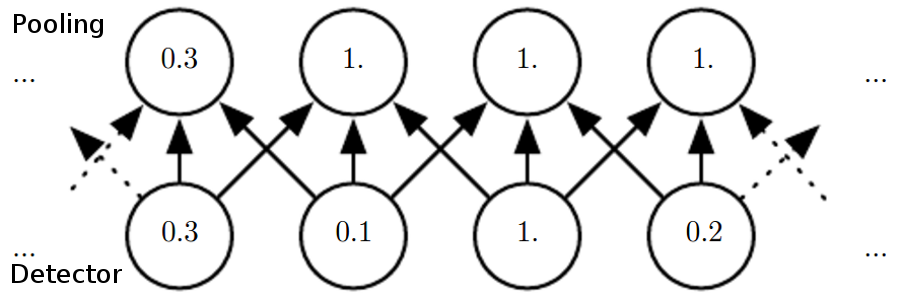
\includegraphics[width=0.7\textwidth]{fig/pool}
  \caption{Operação de \textit{pooling} com região de tamanho 3. Nesta operação é selecionado o máximo valor de ativação da etapa de detecção.}
  \label{fig:pool}
\end{center}
\end{figure}

A operação de \textit{pooling} permite lidar com entradas de tamanho variável.
Classificar imagens de tamanhos diferentes, por exemplo, pode ser realizado
variando o tamanho entre as regiões de \textit{pooling} de modo que a camada de 
de classificação sempre receba o mesmo número de sumários estatísticos
independente do tamanho da imagem.









